\section{导数的计算与核验}
\label{sec:sens-computation}

局部导数的公式已经有了，怎样计算它们，又怎样确认算出的结果可信？

\paragraph{主要思想：一次分解，多个右端}
式~\eqref{eq:sens-inequality-derivative}的系数矩阵$\bm{K}$只依赖基准点，右端$\bm{B}$的每一列对应一个参数。记$N=n+a+p$，把待求的两块Jacobian矩阵合写成
\[
 \bm{Z}=\begin{bmatrix}\bm{D}_{\bm{x}}\\\bm{D}_{\bm{w}}\end{bmatrix}\in\mathbb{R}^{N\times q}.
\]
需要解的是
\begin{equation}
 \bm{K}\bm{Z}=-\bm{B}.
 \label{eq:sens-compute}
\end{equation}
这相当于同一个矩阵配上$q$个右端，只需分解一次，然后对每一列回代。不需要对每个参数重解一次原来的非线性问题。$\bm{K}$对称而不定，通常用带主元选取的$\bm{L}\bm{D}\bm{L}^{\top}$分解，分解的做法可参考\BookChapterRef{chap:direct-linear-solvers}{卷二第12章“线性方程的直接求解”}。

分解还可以顺便检查极小性。$\bm{J}$行满秩时，$\bm{W}$在$\ker\bm{J}$上正定，当且仅当$\bm{K}$恰有$n$个正特征值、$a+p$个负特征值、没有零特征值。这称为\term{惯性}（inertia）判别，证明可查阅\scite{math-nocedal2006numerical}。$\bm{L}\bm{D}\bm{L}^{\top}$分解的$\bm{D}$与$\bm{K}$合同，读出$\bm{D}$的正负特征值个数，就得到惯性，不必另算。

\paragraph{主要思想：只要一个输出时用伴随}
有时我们并不需要整个$\bm{D}_{\bm{x}}$，只要一个标量输出$\phi(\bm{x}(\bm{\theta}))$对$q$个参数的梯度。这时梯度是
\[
 \nabla_{\bm{\theta}}\phi=\bm{D}_{\bm{x}}^{\top}\bm{c},\qquad\bm{c}=\nabla\phi(\bm{x}).
\]
代入式~\eqref{eq:sens-compute}，并在$\bm{c}$后面补零以匹配维数，就是
\begin{equation}
 \nabla_{\bm{\theta}}\phi=-\bm{B}^{\top}\bm{r},\qquad
 \bm{K}\bm{r}=\begin{bmatrix}\bm{c}\\\bm{0}\end{bmatrix}.
 \label{eq:sens-adjoint}
\end{equation}

这里用到$\bm{K}$对称。式~\eqref{eq:sens-adjoint}只解一个线性方程，与参数个数无关。这种做法称为\term{伴随法}（adjoint method）。两种算法的差别只是矩阵乘积$\bm{c}^{\top}\bm{K}^{-1}\bm{B}$的结合顺序不同，见图~\ref{fig:sens-forward-adjoint}。

\begin{BookInlineFigure}
 \centering
 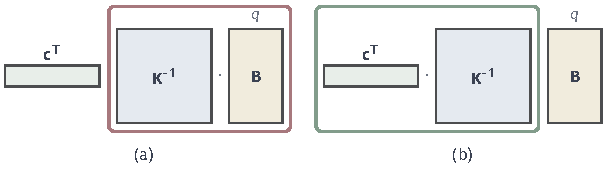
\includegraphics[width=103mm]{figures/05-optimization/06-constrained-optimization/tikz/sens-forward-adjoint/figure.pdf}
 \caption{同一乘积$\bm{c}^{\top}\bm{K}^{-1}\bm{B}$的两种结合顺序。(a)~先算红框内的$\bm{K}^{-1}\bm{B}$，每个参数一个右端，得到全部的$\bm{D}_{\bm{x}}$。(b)~先算绿框内的$\bm{c}^{\top}\bm{K}^{-1}$，只有一个右端，得到单个输出对全部参数的梯度。}
 \label{fig:sens-forward-adjoint}
\end{BookInlineFigure}

表~\ref{tab:sens-cost}比较各种做法的成本，规模变量为$N$与$q$，运算量只计首项。重新求解一列的成本指做一次完整的$\bm{K}$分解，实际的非线性重解通常更贵。$\bm{K}$稀疏时，分解成本由消元产生的填充决定，回代成本是$\bm{L}$的非零元个数的两倍，表中的立方、平方相应缩小，分解一次多次回代的比例关系不变。

\begin{BookInlineTable}
 \centering
 \begin{tabular}{lll}
  \toprule
  做法 & 稠密运算量 & 得到什么\\
  \midrule
  每个参数重解 & $qN^3/3$ & 全部$\bm{D}_{\bm{x}}$\\
  一次分解，$q$次回代 & $N^3/3+2qN^2$ & 全部$\bm{D}_{\bm{x}}$和$\bm{D}_{\bm{w}}$\\
  伴随法 & $N^3/3+2N^2$ & 一个输出的梯度\\
  \bottomrule
 \end{tabular}
 \caption{计算解对参数导数的稠密运算量，$N=n+a+p$。分解的复用要求活动集不变。伴随法的结果再乘$\bm{B}^{\top}$需要的运算量与$\bm{B}$的非零元个数成正比。}
 \label{tab:sens-cost}
\end{BookInlineTable}

\paragraph{计算过程}
下面把全过程用在一个小例子上。预算例中同时考虑两个参数，预算$\tau$和理想点的横坐标偏移$\theta$，基准是$(\tau,\theta)=(2,0)$，目标是
\[
 f(\bm{x},\theta)=\frac12(x_1-2-\theta)^2+\frac12(x_2-1)^2.
\]

\needspace{6\baselineskip}
\paragraph{变量}
\begin{itemize}
 \item 基准解$\bm{x}\in\mathbb{R}^n$，活动乘子与等式乘子合写成$\bm{w}\in\mathbb{R}^{a+p}$。
 \item 系数矩阵$\bm{K}\in\mathbb{R}^{N\times N}$，右端$\bm{B}\in\mathbb{R}^{N\times q}$，$N=n+a+p$。
 \item 输出$\bm{Z}$，形状是$N\times q$，含$\bm{D}_{\bm{x}}$与$\bm{D}_{\bm{w}}$两块。
 \item 每个不活动约束的余量，每个活动约束的乘子，它们决定分支的有效范围。
\end{itemize}

\paragraph{初始化}
先把基准问题求解到足够高的精度，读出解和乘子，再分出活动约束。

例中$n=2$，$a=1$，$p=0$，$q=2$。基准解和乘子是
\[
 \bm{x}=\begin{bmatrix}3/2\\1/2\end{bmatrix},\qquad\lambda_1=\frac12,\qquad A=\{1\}.
\]

\paragraph{计算步骤}
\begin{enumerate}
 \item 组装$\bm{K}$和$\bm{B}$，公式见式~\eqref{eq:sens-inequality-derivative}。

 例中Lagrange函数的梯度和活动约束分别是
 \[
  \nabla_{\bm{x}}\mathcal{L}=(x_1-2-\theta+\lambda_1,\ x_2-1+\lambda_1),\quad g_1=x_1+x_2-\tau,
 \]
 对$\bm{x}$、$\lambda_1$和$(\tau,\theta)$分别求偏导，得到
 \[
  \bm{K}=\begin{bmatrix}1&0&1\\0&1&1\\1&1&0\end{bmatrix},\qquad
  \bm{B}=\begin{bmatrix}0&-1\\0&0\\-1&0\end{bmatrix}.
 \]
 $\bm{B}$的第一列对应$\tau$，第二列对应$\theta$。

 \item 分解$\bm{K}=\bm{L}\bm{D}\bm{L}^{\top}$，并由$\bm{D}$的符号检查惯性。

 例中不需要主元交换，消元得到
 \[
  \bm{L}=\begin{bmatrix}1&0&0\\0&1&0\\1&1&1\end{bmatrix},\qquad
  \bm{D}=\operatorname{diag}(1,1,-2).
 \]
 $\bm{D}$有两个正数和一个负数，与$n=2$，$a=1$相符，这个解是局部极小点。

 \item 对$\bm{B}$的每一列回代，得到$\bm{Z}$的相应列，公式见式~\eqref{eq:sens-compute}。

 例中$\tau$列的右端是$(0,0,1)^{\top}$。依次解$\bm{L}\bm{y}=(0,0,1)^{\top}$、$\bm{D}\bm{y}'=\bm{y}$、$\bm{L}^{\top}\bm{z}=\bm{y}'$，中间结果和最终结果是
 \[
  \bm{y}=\begin{bmatrix}0\\0\\1\end{bmatrix},\quad
  \bm{y}'=\begin{bmatrix}0\\0\\-1/2\end{bmatrix},\quad
  \bm{z}=\begin{bmatrix}1/2\\1/2\\-1/2\end{bmatrix}.
 \]

 $\theta$列的右端是$(1,0,0)^{\top}$，同样回代，得到
 \[
  \bm{y}=\begin{bmatrix}1\\0\\-1\end{bmatrix},\quad
  \bm{y}'=\begin{bmatrix}1\\0\\1/2\end{bmatrix},\quad
  \bm{z}=\begin{bmatrix}1/2\\-1/2\\1/2\end{bmatrix}.
 \]

 \item 用余量和乘子确定有效范围。把导数代入，对方向$(\Delta\tau,\Delta\theta)$写出需要保持为正的量。

 例中这三个量分别是
 \[
  \begin{aligned}
  \lambda_1&=\frac12-\frac12\Delta\tau+\frac12\Delta\theta,\\
  x_1&=\frac32+\frac12\Delta\tau+\frac12\Delta\theta,\\
  x_2&=\frac12+\frac12\Delta\tau-\frac12\Delta\theta.
  \end{aligned}
 \]
 它们都大于零的区域是参数平面上的一个多面体，图~\ref{fig:sens-critical-regions}中绿色的带形就是这个区域在图中范围内的部分。

 \item 给出预测，并用小幅参数重求解核验：预测的活动集是否保持，预测的解与重解的结果相差多少。

 例中取$(\Delta\tau,\Delta\theta)=(0.2,0.1)$，三个量都为正，预测和重解都是
 \[
  \bm{x}=(1.65,\ 0.55),\qquad\lambda_1=0.45.
 \]
 问题在这个活动集上是二次的，所以预测是精确的。若取$(\Delta\tau,\Delta\theta)=(-1.5,0)$，预测给出$x_2=-1/4<0$，这说明活动集已经改变，需要换到活动集$\{1,3\}$重新计算，真实解是$(0.5,0)$。
\end{enumerate}

整个计算是一次完成的，没有迭代，到步骤五结束。最终得到
\[
 \bm{D}_{\bm{x}}=\begin{bmatrix}1/2&1/2\\1/2&-1/2\end{bmatrix},\qquad
 \bm{D}_{\lambda_1}=\begin{bmatrix}-1/2&1/2\end{bmatrix}.
\]

\begin{BookInlineFigure}
 \centering
 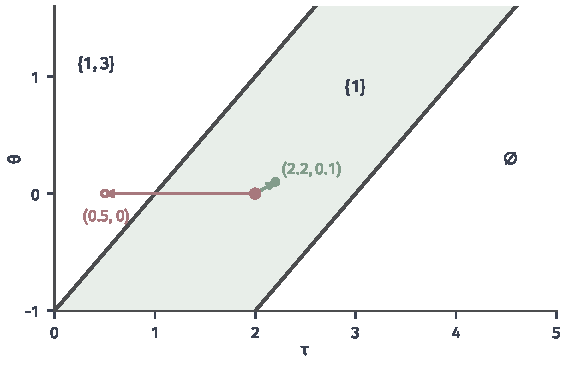
\includegraphics[width=96mm]{figures/05-optimization/06-constrained-optimization/matplotlib/sens-critical-regions/figure.pdf}
 \caption{参数平面$(\tau,\theta)$上的活动集区域。两条深灰线是$\tau=1+\theta$和$\tau=3+\theta$，它们划分出活动集$\{1,3\}$、$\{1\}$和$\varnothing$。红点是基准$(2,0)$，绿色箭头走到同一区域内的$(2.2,0.1)$，一阶预测有效；红色箭头越过边界到$(0.5,0)$，一阶预测失效。}
 \label{fig:sens-critical-regions}
\end{BookInlineFigure}

伴随法在这个例子上也可以手算。设只关心输出$\phi=x_2$，$\bm{c}=(0,1)^{\top}$。由式~\eqref{eq:sens-adjoint}，解$\bm{K}\bm{r}=(0,1,0)^{\top}$，得到$\bm{r}=(-1/2,1/2,1/2)^{\top}$，再求
\[
 \nabla_{(\tau,\theta)}x_2=-\bm{B}^{\top}\bm{r}=\begin{bmatrix}1/2\\-1/2\end{bmatrix}.
\]
这正是$\bm{D}_{\bm{x}}$的第二行，一次回代就得到了两个参数的结果。

\paragraph{算法分析：误差的三个来源}
隐式导数的公式对应精确的最优性方程。实际算出的导数还带有三种误差，它们的性质不同。

第一种是近似解带来的误差。基准解只解到$\tilde{\bm{x}}$，$\bm{K}$和$\bm{B}$都在$\tilde{\bm{x}}$处组装，导数的误差与解的误差成正比，比例系数由$\bm{K}^{-1}$和二阶导数的变化率决定。参数只出现在线性项时$\bm{B}$不依赖于$\bm{x}$，二次目标下这项误差为零。

第二种是有限差分的误差。用重解来核验导数时，常用中心差分
\[
 \frac{\bm{x}(\bm{\theta}+h\bm{d})-\bm{x}(\bm{\theta}-h\bm{d})}{2h},
\]
截断误差是$O(h^2)$。若每次重解的误差是$\varepsilon$，差分会放大成$O(\varepsilon/h)$。两项相加的误差在$h\sim\varepsilon^{1/3}$时最小，约为$\varepsilon^{2/3}$。

第三种是算法展开的误差。把迭代算法写成关于$\bm{\theta}$的函数，对$T$步迭代逐步求导，得到的是$\bm{x}^{(T)}$的导数，而不是$\bm{x}^\star$的导数。以梯度下降为例，它的迭代是
\[
 \bm{x}^{(t+1)}=\bm{x}^{(t)}-\alpha\nabla_{\bm{x}}f(\bm{x}^{(t)},\bm{\theta}),
\]
导数的递推式是
\begin{equation}
 \bm{D}^{(t+1)}=\bigl(\bm{I}-\alpha\nabla^2_{\bm{x}\bm{x}}f\bigr)\bm{D}^{(t)}-\alpha\nabla^2_{\bm{x}\bm{\theta}}f,
 \label{eq:sens-unroll}
\end{equation}
其中各导数都在$(\bm{x}^{(t)},\bm{\theta})$处取值。它的不动点正是式~\eqref{eq:sens-unconstrained-derivative}。

图~\ref{fig:sens-fd-unroll}用具体计算展示了这些误差。(a)中，差分误差先随$h$减小而减小，到某个$h$之后反而增大，这个转折点随求解精度$\varepsilon$移动。(b)在岭回归例子上比较了式~\eqref{eq:sens-unroll}的展开和在当前迭代点上计算的隐式导数：$\gamma$改变了曲率，展开的误差多了一个随$t$增长的因子，所以比隐式导数略慢。

\begin{BookInlineFigure}
 \centering
 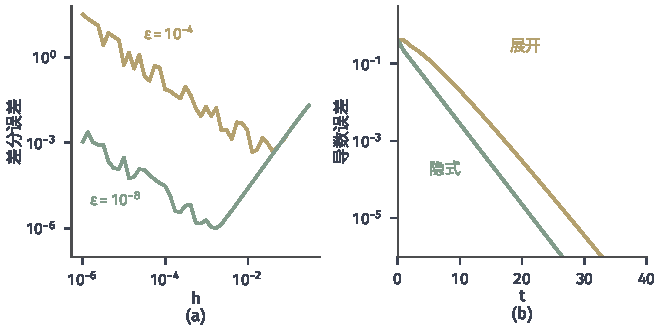
\includegraphics[width=112mm]{figures/05-optimization/06-constrained-optimization/matplotlib/sens-fd-unroll/figure.pdf}
 \caption{导数计算的误差。(a)~价格例$\theta=1$处$x_2$对$\theta$的中心差分误差。每次重解用梯度下降到残差$\varepsilon$，曲线取$40$次随机起点的中位数，黄线$\varepsilon=10^{-4}$，绿线$\varepsilon=10^{-8}$。(b)~岭回归例$\gamma=1$，步长$\alpha=1/L$，黄线是展开$t$步梯度下降得到的导数的误差，绿线是在$\bm{x}^{(t)}$处计算隐式导数的误差。}
 \label{fig:sens-fd-unroll}
\end{BookInlineFigure}

\paragraph{算法分析：非二次问题的核验}
第~\ref{sec:sens-general-constraints}节的价格例不是二次的，一阶预测有误差，可以检验误差的阶。在$\theta=1$处，由$\lambda'(1)=1$，$x_1'=1-\lambda-\lambda'\theta=-1/2$，$x_2'=-\lambda'=-1$。与重解的结果比较，
\[
 \begin{aligned}
 h&=0.1:\quad \bm{x}=(1.4480,\ 0.4072),\quad\text{预测}\ (1.45,\ 0.4),\\
 h&=0.01:\quad \bm{x}=(1.49498,\ 0.49007),\quad\text{预测}\ (1.495,\ 0.49).
 \end{aligned}
\]
误差分别约为$7.5\times10^{-3}$和$7.9\times10^{-5}$，$h$缩小十倍，误差缩小约一百倍，与二阶截断误差一致。

这个一致性只在活动集保持时成立。价格例的预算活动窗口是$(\sqrt{5}-1)/2<\theta<2$，$\theta>2$时$x_2\geq0$起作用。图~\ref{fig:sens-prediction-error}(b)中，$h$接近$1$时误差开始偏离$h^2$的规律。检验时还应比较左右两侧的差商，它们不相等，或者差商不随$h$收敛，常常说明活动集正在改变。

\begin{BookInlineFigure}
 \centering
 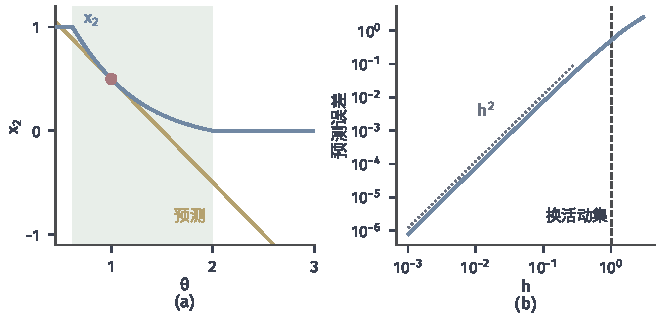
\includegraphics[width=112mm]{figures/05-optimization/06-constrained-optimization/matplotlib/sens-prediction-error/figure.pdf}
 \caption{价格例的一阶预测。(a)~$x_2(\theta)$的真实值（蓝线）和$\theta=1$处的线性预测（黄线），绿色区域是活动集保持的窗口。(b)~预测误差随$h$的变化（对数坐标，$\theta=1+h$），灰色点线是$h^2$的参考线，黑色虚线标出活动集改变的位置$h=1$。}
 \label{fig:sens-prediction-error}
\end{BookInlineFigure}
